\chapter{\label{sec:introduction}Introduction}

Over recent years, the continuing increase in available computing power, coupled with the public's ever-increasing thirst for entertainment, has made the use of three-dimensional computer graphics commonplace. From film and television production, through to games and Internet-based shopping, the demand for highly realistic 3D content is increasing at an enormous rate. The computing power available to display such 3D content doubles roughly every 18 months, in line with Moore's Law, a trend which shows no sign of abating. Today's personal computers are capable of creating images more realistic than was possible with the most advanced supercomputers 10 years ago (see figure \ref{fig:3dgraphics} for some examples).

\begin{figure}
\begin{center}
\begin{tabular}{ccc}
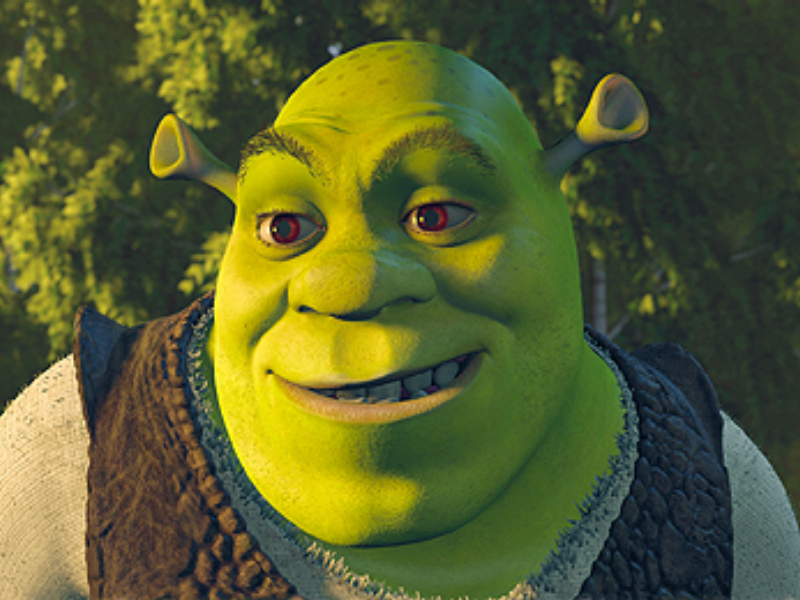
\includegraphics[width=4.7cm]{../images/shrek} &
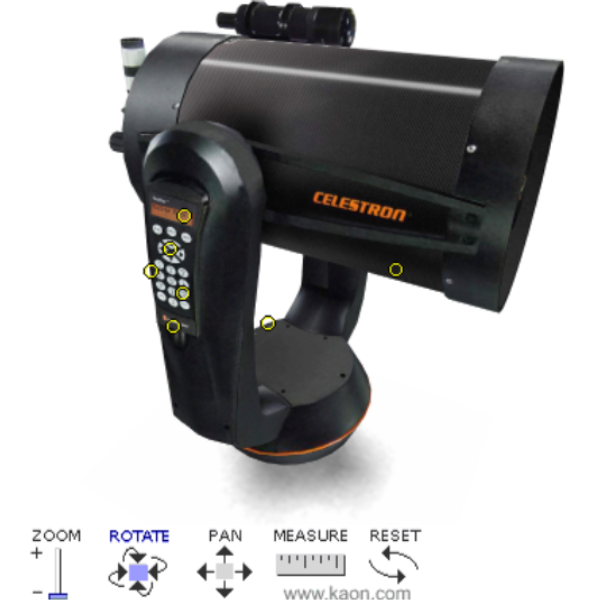
\includegraphics[width=3.5cm]{../images/kaon} &
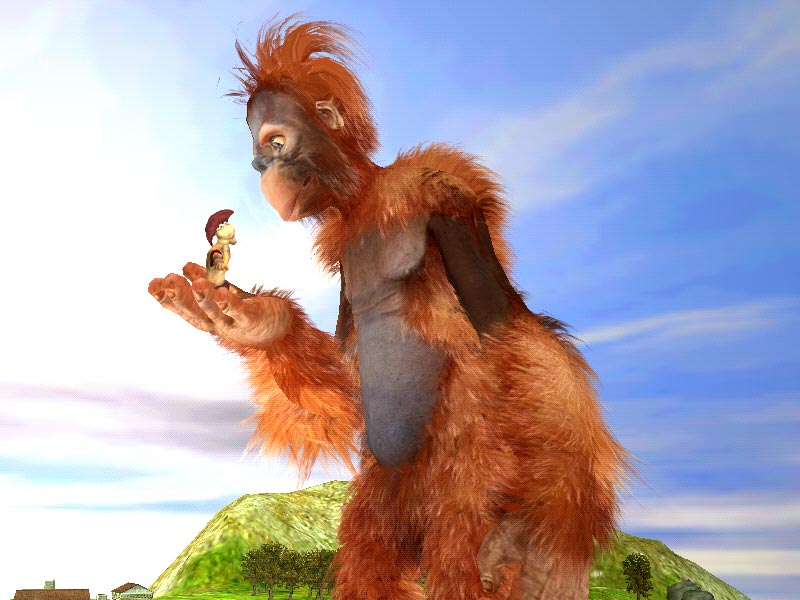
\includegraphics[width=4.7cm]{../images/black_white} \\
{\it (a)} & {\it (b)} & {\it (c)}
\end{tabular}
\caption[Uses of 3D Graphics]{\label{fig:3dgraphics} Uses of 3D Graphics. (a) Film: a still from {\it Shrek} from PDI/Dreamworks\cite{PDI}. (b) Online: 3D product visualisation by Kaon\cite{Kaon}. (c) Games: a screenshot from {\it Black \& White 2}, by Lionhead Studios\cite{Lionhead}.}
\end{center}
\end{figure}

\section{\label{sec:introduction:contentcreation}3D Content Creation}

The 3D content creation process however, has not kept pace with this explosion in visualisation capabilities. One of today's major challenges is to create models that have highly detailed, realistic surfaces, but can also be animated realistically. The process of creating realistic 3D content is still extremely time consuming, even for skilled artists. Therefore, in order to keep pace with the demand that the hardware and the public have for 3D content, we require new methods of content creation which are faster and more highly automated than traditional modelling techniques. We must also consider methods for efficient transport and delivery of this realistic content, as network bandwidth will always lag behind the capabilities of computer hardware to process such data.

Within the field of 3D content creation, one particular problem is the creation of accurate models of real-world objects. Such models can be created using one of two methods - either they can be created from scratch by an artist using a 3D modelling tool such as 3D Studio MAX or Maya, or alternatively, object scanning hardware can be used to capture the surface. 

The first method is wholly manual, extremely time-consuming, and requires a large amount of skill on the part of the content creator. The second method lends itself to automation, potentially reducing the skill and time required to create a realistic model. Advances in 3D sensor technology have provided an efficient way to capture photo-realistic 3D models of real objects. However, such reconstructed surface models are usually composed of a dense, unstructured polygonal mesh representing the surface detail of the object at the full resolution and accuracy of the sensor. As noted by \citet{Thalmann96}, such meshes are notoriously expensive to store, transmit, and render, and in particular are extremely awkward to animate. The goal of this research is to enable the creation of high-quality models based on captured surface data, that can also be animated efficiently \cite{Sun99}.

We discuss the state of the art for the problem of animating such dense surface data in Chapter \ref{sec:litreview}. In particular we discuss prior art in model capture and animation, focusing in particular on 3D capture systems, model representations, character animation, and compression of 3D data.

\section{\label{sec:introduction:layered}Layered Models}

\begin{figure}
\begin{center}
\begin{tabular}{cccc}
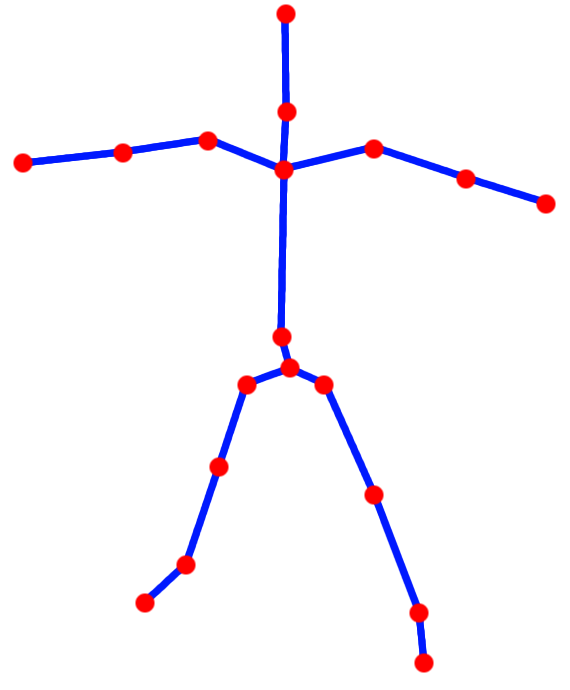
\includegraphics[width=4.4cm]{../images/skeleton_layer} &
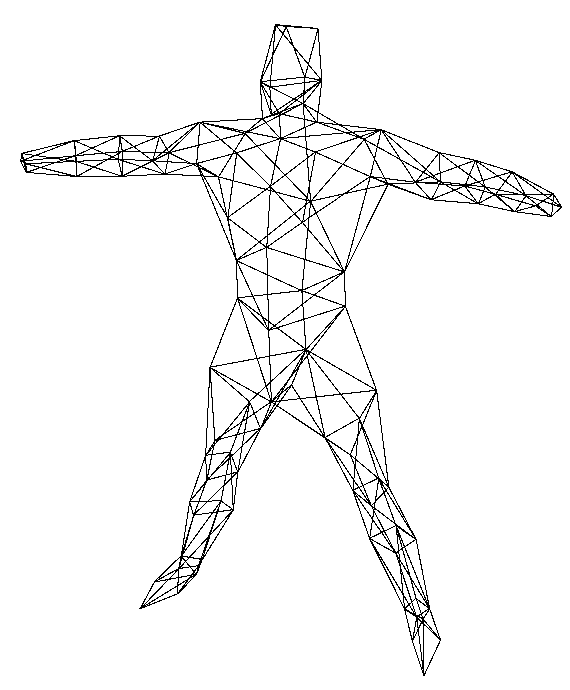
\includegraphics[width=4.4cm]{../images/control_layer} &
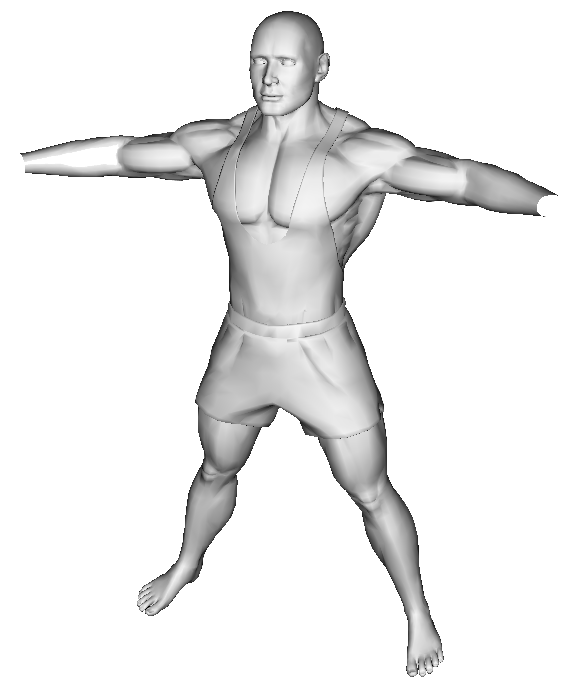
\includegraphics[width=4.4cm]{../images/detail_layer} \\
{\it(a)} & {\it(b)} & {\it(c)}
\end{tabular}
\caption[Layered Models]{\label{fig:layeredmodel} Layered Models (a) Skeleton Layer  (b) Control Layer  (c) Detail Layer}
\end{center}
\end{figure}

Typically, surface models reconstructed from captured data are composed of millions of polygons, and the articulation structure of the object is unknown. Animating such datasets directly is computationally expensive and it is difficult to achieve a realistic result. 

In order to solve this problem, we introduce methods for reconstructing {\it layered models} from captured data, which facilitate realistic animation. The model consists of a number of separate layers, each of which performs a different animation task; in particular, the layered model allows an animator to manipulate a low-resolution version of the model in real-time and render the full surface detail offline to achieve full quality output.

This approach provides a relatively fast and simple technique for building animated models from captured surface measurements. The resulting model gives an efficient, realistic animation of the detailed surface, while providing a low-resolution control structure for real-time interactive animation. The method can also be extended to allow many extra applications, such as variable level-of-detail rendering and model compression.

\subsection{\label{sec:introduction:layered:skeletal}Skeletal Animation}
\nomenclature{\bf Skeleton}{A hierarchical articulation structure, which can be used to drive animation of a detailed surface.}
The lowest layer in our system is a {\it skeleton layer} (see figure \ref{fig:layeredmodel}a). A hierarchical skeleton structure is fitted interactively to the mesh, and can then be animated using common animation techniques such as keyframing, inverse kinematics, physics-based models, or motion capture. The use of a skeleton layer greatly simplifies the process of animating the captured model, as the motion of the skeleton, which is easily defined, can be used to provide control of all the higher layers. In chapter {\ref{sec:skeletalanim}, we present a novel skeletal animation technique which requires minimal operator input during the creation phase, and we also present a complete implementation of this animation system in VRML.

\subsection{\label{sec:introduction:layered:control}The Control Layer}
\nomenclature{\bf Control Layer}{A mesh representation of an object containing a relatively low number of polygons.}
The middle layer is a low-resolution {\it control layer} (see figure \ref{fig:layeredmodel}b). Although the skeleton alone would be sufficient for motion control of the scanned data, it is too simple to be used as a representation of an object during animation design. For instance, a skeleton model would be unsuitable for collision detection or accurate targeting for inverse kinematics systems. On the other hand, the high-resolution model is prohibitively expensive to work with. Therefore it is desirable to introduce an intermediate layer. This control layer is a representation of the object with the same basic shape and topology as the captured data, but a much lower polygon count. This control layer can be a simplification of the captured data, a completely separate generic model, for instance a box-like model such as Discreet's Biped from 3D Studio MAX\cite{3DSMAX}, or a more complex structured model such as those available from Viewpoint\cite{Viewpoint}. This control layer is mapped to the skeleton layer, enabling its animation to be driven by movements of the skeleton structure. The process of mapping the control layer to the skeleton layer, and using this mapping to animate the control layer mesh based on skeletal motion is discussed in detail in chapter \ref{sec:skeletalanim}, as part of our discussion of skeletal animation. 

\subsection{\label{sec:introduction:layered:scandata}Animation of Dense Scanned Data}
\nomenclature{\bf Detail Layer}{A complex polygon mesh representing the surface of a scanned object at the maximum level of detail measured.}
The topmost layer in our model is the {\it detail layer} (shown in figure \ref{fig:layeredmodel}c). This layer is composed of the original high-resolution captured data, and is used in the final full-quality rendering stage of production, to reconstruct an accurate surface for the object. The detail layer is mapped to the control layer, allowing control layer animation to drive changes in the geometry of the detail layer. In chapter \ref{sec:scandata}, we present the mapping and animation methods which, when taken together with the aforementioned skeletal animation of the control layer, allow us to apply skeletal animation techniques to dense scanned surface data. 

\section{\label{sec:introduction:dispmaps}Displacement Maps}
\nomenclature{\bf Displacement Map}{A 2D image in which each pixel represents a displacement value for the surface of a control layer at the corresponding texture coordinate.}
\nomenclature{\bf Texture Map}{A coloured 2D image that is mapped onto a surface to represent details that are not present in the geometry of the surface.}
\begin{figure}
\begin{center}
\begin{tabular}{cc}
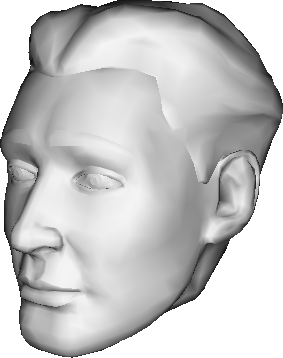
\includegraphics[height=5cm]{../images/cubehead_detail} &
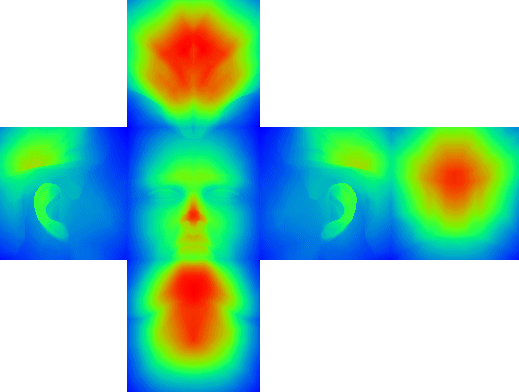
\includegraphics[height=5cm]{../images/cubehead_full} \\
{\it (a)} & {\it (b)}
\end{tabular}
\caption[Displacement Mapping]{\label{fig:dispmaps} Displacement Mapping. The detailed model shown in (a) can be represented as the displacement map shown in (b). The displacement map has been colourised to enhance the visibility of details. }
\end{center}
\end{figure}
The layered animation method described above allows us to animate dense datasets easily. However, it still requires animation and rendering of the full dataset, which may be too computationally expensive for anything but offline rendering. We therefore present an alternative representation of the detail layer using {\it displacement maps}. The detail layer is represented as a continuous 2D function across the surface of the control layer, which can be stored in an image form, similar to a texture mapped polygon mesh. An example is shown in figure \ref{fig:dispmaps}. This representation has a number of potential advantages, including variable level-of-detail rendering, simple editing, and geometry compression. The process of creating a displacement map for a detail layer is discussed in chapter \ref{sec:dispmapcreation}. Reconstruction and animation of displacement mapped models, as well as editing and compression, are discussed in chapter \ref{sec:dispmapanim}.

\section{\label{sec:introduction:whodidwhat}Division of Labour}

The techniques and algorithms discussed in this thesis were developed in conjunction with Adrian Hilton, Wei Sun, and Gordon Collins of the University of Surrey. In the areas where I did not carry out the majority of the work myself, it will be made clear in the text.

\section{\label{sec:introduction:publications}Publications}

As well as this thesis, the layered animation and displacement mapping methods have been presented in a number of published papers.

\begin{itemize}
\item{\bibentry{Sun99}}.
\item{\bibentry{Smith00}}.
\item{\bibentry{Sun00}}.
\item{\bibentry{Smith00a}}.
\item{\bibentry{Sun01}}.
\item{\bibentry{Starck03}}.
\end{itemize}
